\documentclass[english,14pt]{beamer}
\usetheme{EastLansing}
\usecolortheme{spruce}

\usepackage{xcolor}
\usepackage{listings}
\usepackage{courier}
\usepackage{graphicx}
\usepackage{amsmath}
\usepackage{algorithm2e}
\usepackage{multicol}
\usepackage{hyperref}
\usepackage{textcomp}

% http://mirrors.ibiblio.org/CTAN/macros/latex/contrib/datetime2/datetime2.pdf
\usepackage{babel}
\usepackage[useregional]{datetime2}

% https://tex.stackexchange.com/questions/42619/x-mark-to-match-checkmark
\usepackage{pifont}% http://ctan.org/pkg/pifont

%% https://stackoverflow.com/questions/1435837/how-to-remove-footers-of-latex-beamer-templates
%%gets rid of bottom navigation bars
%\setbeamertemplate{footline}[page number]
%
%gets rid of navigation symbols
\setbeamertemplate{navigation symbols}{}


\usefonttheme[onlymath]{serif}

\definecolor{mGreen}{rgb}{0,0.6,0}
\definecolor{mGray}{rgb}{0.5,0.5,0.5}
\definecolor{mPurple}{rgb}{0.8,0,0.82}
\definecolor{backgroundColour}{rgb}{0.95,0.95,0.92}
\definecolor{lightBlue}{rgb}{0.1, 0.1, 0.8}

\newcommand\red[1]{{\color{red} #1}}
\newcommand\green[1]{{\color{green} #1}}
\newcommand\blue[1]{{\color{blue} #1}}

\newcommand{\cmark}{\ding{51}}%
\newcommand{\xmark}{\ding{55}}%

\lstdefinestyle{CStyle}{
    backgroundcolor=\color{backgroundColour},   
    commentstyle=\color{mGreen},
    keywordstyle=\color{magenta},
    numberstyle=\tiny\color{mGray},
    stringstyle=\color{mPurple},
    basicstyle=\footnotesize,
    breakatwhitespace=false,         
    breaklines=true,                 
    captionpos=b,                    
    keepspaces=true,                 
    numbers=left,                    
    numbersep=5pt,                  
    showspaces=false,                
    showstringspaces=false,
    showtabs=false,                  
    tabsize=2,
    language=Python
}

\lstdefinestyle{pseudo}{
        basicstyle=\ttfamily\footnotesize,
        keywordstyle=\color{lightBlue},
        morekeywords={BEGIN,END,IF,ELSE,ENDIF,ELSEIF,PRINT,WHILE,RETURN,ENDWHILE,DO,FOR,TO,IN,ENDFOR,BREAK,INPUT,CONDITIONS},
        morecomment=[l]{//},
        commentstyle=\color{mGreen}
}

\lstset{basicstyle=\footnotesize\ttfamily,breaklines=true}
\lstset{framextopmargin=50pt,tabsize=2}

\title{ENGG1003 - Monday Week 8}
\subtitle{Solving nonlinear algebraic equations }%\\ \& computing integrals}
\author{Steve Weller}
\institute{University of Newcastle}
%\date{\today}
\date{26 April 2021}

% following is a bit of a hack, but forces page numbers (technically: frame numbers) to run 1,2,3,... 
% with titlepage counting as frame 1

\addtocounter{framenumber}{1}
\titlepage

\begin{document}

\begin{flushleft}
{\scriptsize Last compiled:~\DTMnow}
\vspace*{-5mm}
\end{flushleft}
\framebreak

%==============================================================

\begin{frame}[fragile]

\frametitle{Lecture overview}
\begin{enumerate}
	\item Solving nonlinear algebraic equations \red{pp.~175-176}
	\begin{itemize}
		\item general setting
		\item problem: fluid level in measuring cup
	\end{itemize}
	
	\item[]
	
	\item Bisection method \red{\S7.4}
	
	\item[]
	
	\item Secant method \red{\S7.3}
	\begin{itemize}
		\item Newton's method
	\end{itemize}
	
	\item[]
	
	\item Extensions
	\begin{itemize}
		\item bisection \& secant methods: re-write as functions
		\item timing code in Python
		\item speed comparisons: bisection vs.~secant
	\end{itemize}
	
\end{enumerate}

\end{frame}

%==============================================================

\begin{frame}[fragile]

\frametitle{$1)$ Solving nonlinear algebraic equations}

\begin{itemize}
	\item \red{\emph{linear}} equations: $ax + b = 0$
	\begin{itemize}
		\item solution $x = -b/a$
	\end{itemize}
	\item[]
	\item \red{\emph{nonlinear}} equations
	\begin{itemize}
		\item quadratic $ax^2 + bx+c = 0$: solution $x = \frac{-b \pm\sqrt{b^2-4ac}}{2a}$
		\item cubic and quartic (orders $3$ and $4$): exact solutions exist but are \emph{very} complicated
		\item quintic (order $5$) equations: exact solutions \emph{do not exist} in general, proving that needs \emph{serious} mathematics
	\end{itemize}
	\item[]
	\item most equations in engineering applications have no exact ``pen and paper'' solutions!
	
	
\end{itemize}

\end{frame}

%==============================================================

\begin{frame}[fragile]

\frametitle{Numerical solutions to equations}

\begin{flushright}
\small\emph{``Far better an approximate answer to the right question\ldots \\ than an exact answer to the wrong question''}\\---John Tukey
\end{flushright}
\vspace*{-3mm}
\textbf{General problem:} find $x$ satisfying
	\[
		f(x) = 0
	\]
	where $f(x)$ is a formula involving $x$
	
	\textbf{Example}
	\[
		f(x) = e^{-x}\sin(x) - \cos(x)
	\]
	has solution $x = 7.85359326$ because
	\[
	e^{-7.85359326}\sin(7.85359326) - \cos(7.85359326) = 0.000
	\]

\end{frame}

%==============================================================

\begin{frame}[fragile]

\frametitle{Fluid level in truncated cone}

\vspace*{-3mm}
\begin{figure}[ht]
	\centering
	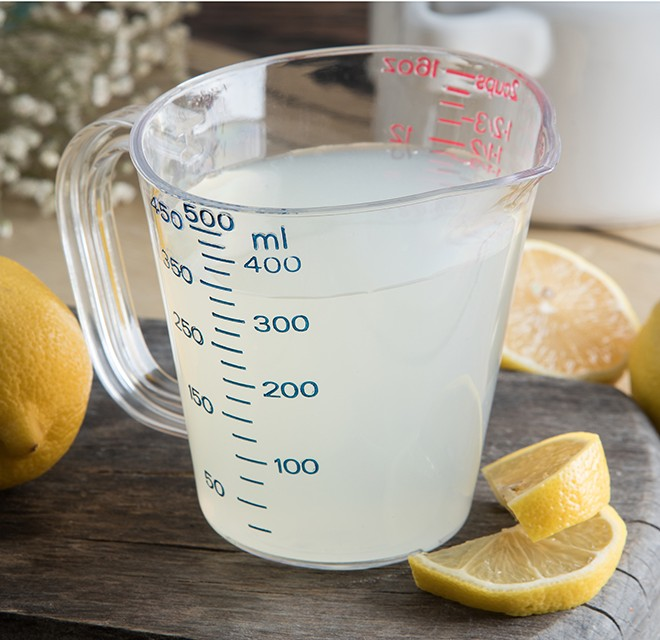
\includegraphics[width=0.45\textwidth]{figures/measuringCup}\hspace*{2mm}%
	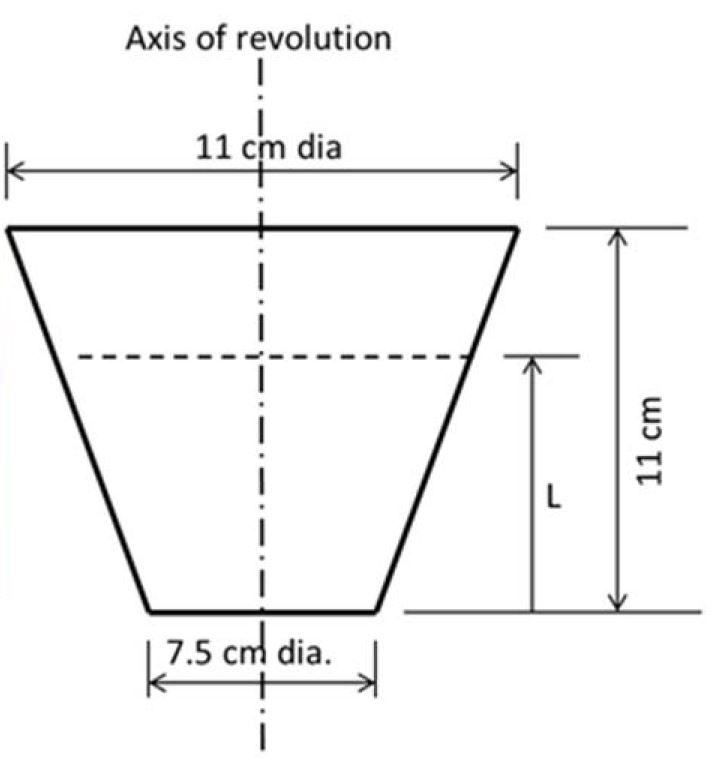
\includegraphics[width=0.45\textwidth]{figures/cupDimensions}
\end{figure}

\begin{itemize}
	\item applications: water in dam, coal in conical hopper
\end{itemize}

\end{frame}

%==============================================================

\begin{frame}[fragile]

\frametitle{Fluid level}

\vspace*{-4mm}
\begin{figure}[ht]
	\centering
	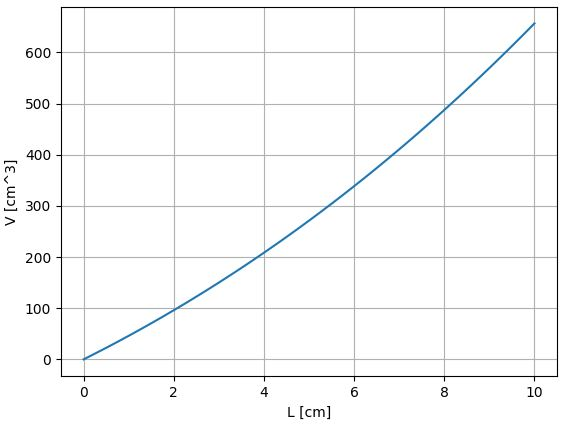
\includegraphics[width=0.6\textwidth]{figures/fluidVvsL}
\end{figure}
\vspace*{-4mm}
\begin{itemize}
	\item volume $V$ depends on depth $L$ as follows: %, \emph{presented without proof:}
	\[
		V = 0.0268L^3 + 1.884L^2 + 44.15L
	\]
	\vspace*{-4mm}
	\begin{itemize}
		\item $V$ (in millilitres, mL),  $L$ (in cm) 
	\end{itemize}
\end{itemize}
	
\end{frame}

%==============================================================

\begin{frame}[fragile]

\frametitle{Fluid level}

\vspace*{-4mm}
\begin{figure}[ht]
	\centering
	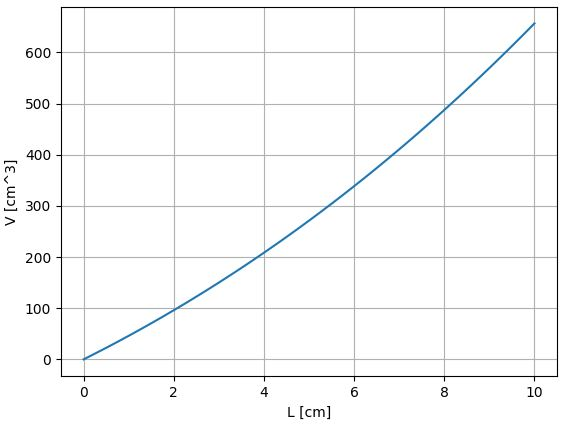
\includegraphics[width=0.5\textwidth]{figures/fluidVvsL}
\end{figure}
\vspace*{-4mm}
\begin{itemize}
	\item[] \textbf{Q: depth $L$ when cup holds $500$~mL of water?}
	\item need to solve equation
	\[
	500 = 0.0268L^3 + 1.884L^2 + 44.15L
	\]
	$f(L) = 0.0268L^3 + 1.884L^2 + 44.15L - 500 = 0$
\end{itemize}
	
\end{frame}

%==============================================================

\begin{frame}[fragile]

\frametitle{$2)$ Bisection method}

\vspace*{-15mm}
\begin{figure}[ht]
	\centering
	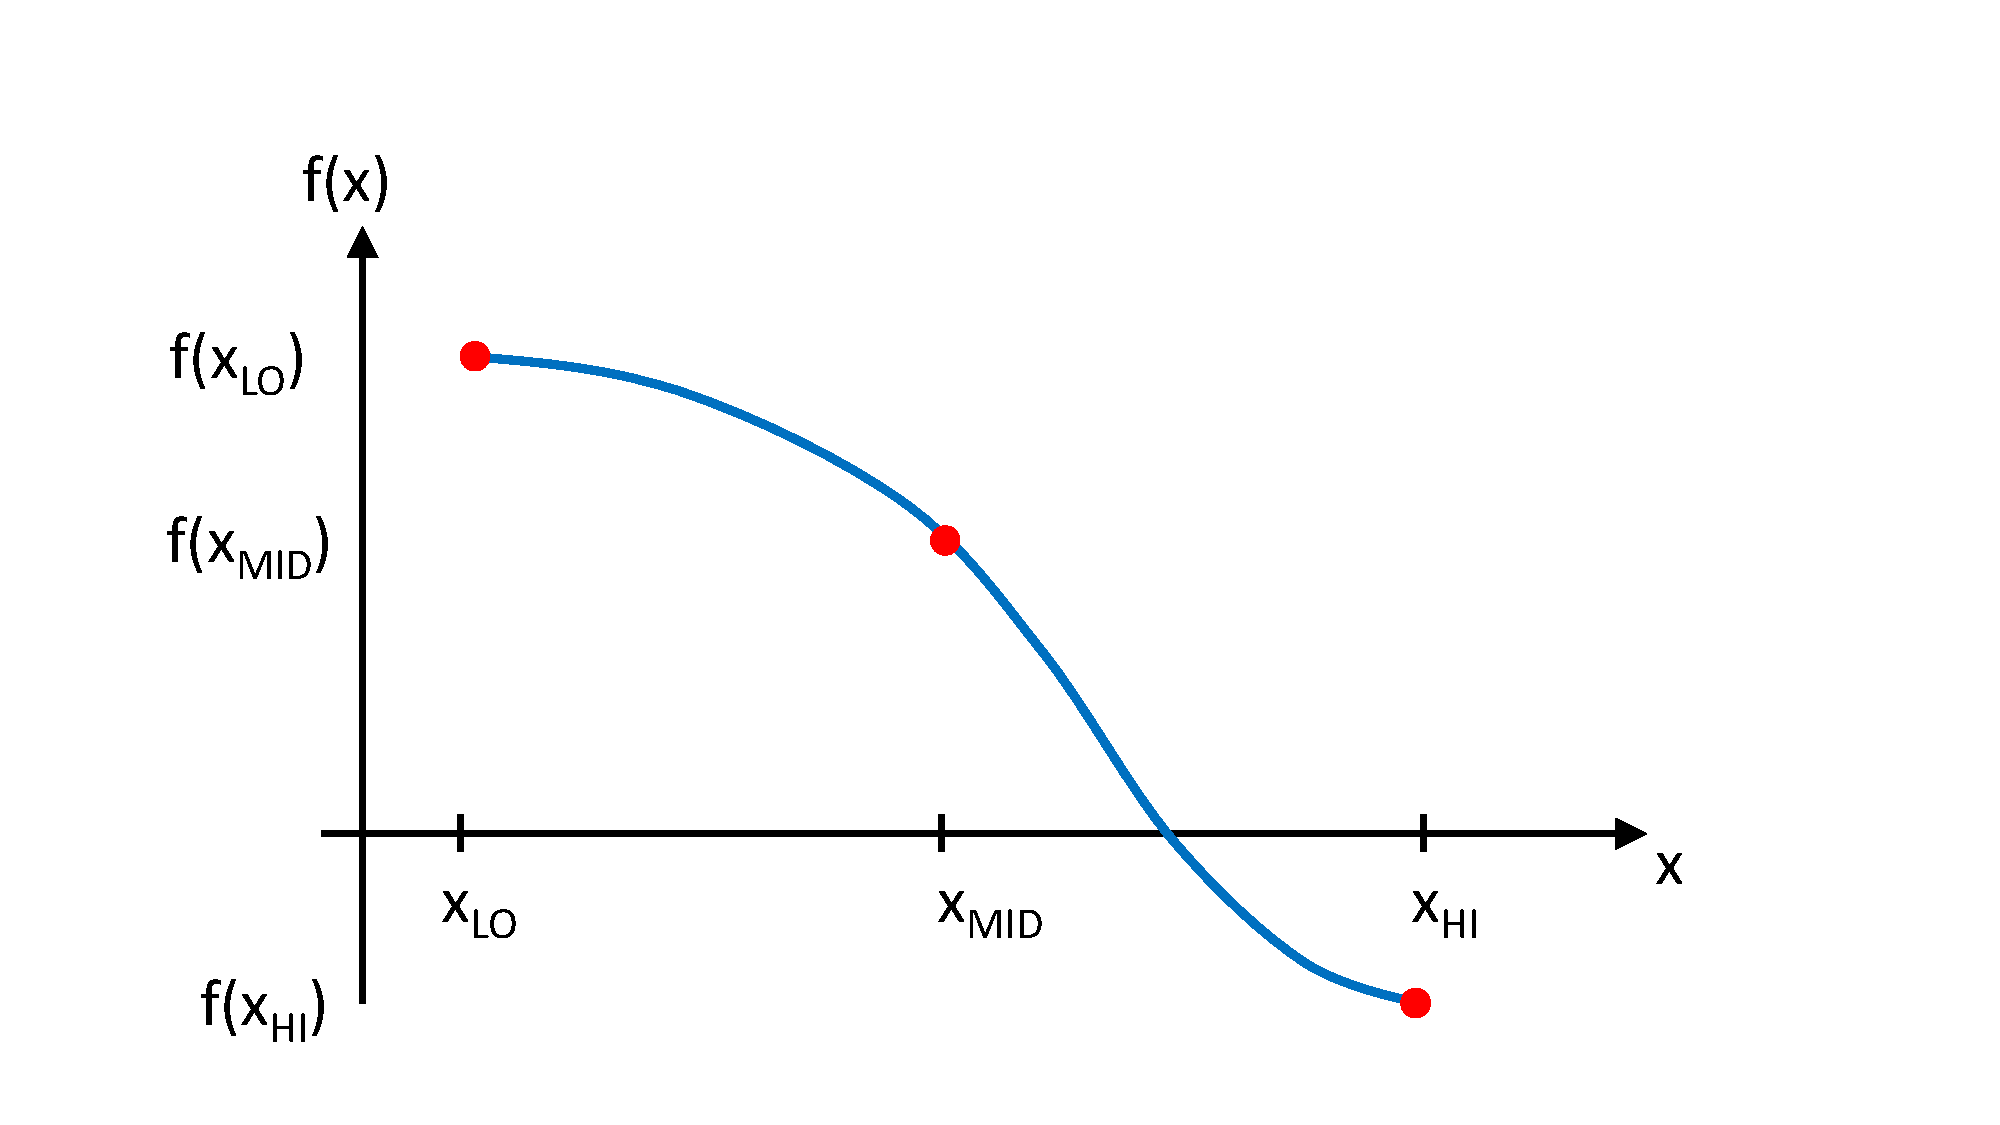
\includegraphics[width=0.8\textwidth]{figures/bisection1}
\end{figure}
\vspace*{-10mm}
\begin{itemize}
\item continuous function $f(x)$ on interval $[x_\mathrm{LO},x_\mathrm{HI}]$, where value of $f$ \emph{changes sign} from $x_\mathrm{LO}$ to $x_\mathrm{HI}$
\item divide interval in two, $f(x)=0$ in one sub-interval
\item select sub-interval where sign of $f$ changes \& repeat
\end{itemize}

\end{frame}

%==============================================================

\begin{frame}[fragile]

\frametitle{Bisection method}

\vspace*{-15mm}
\begin{figure}[ht]
	\centering
	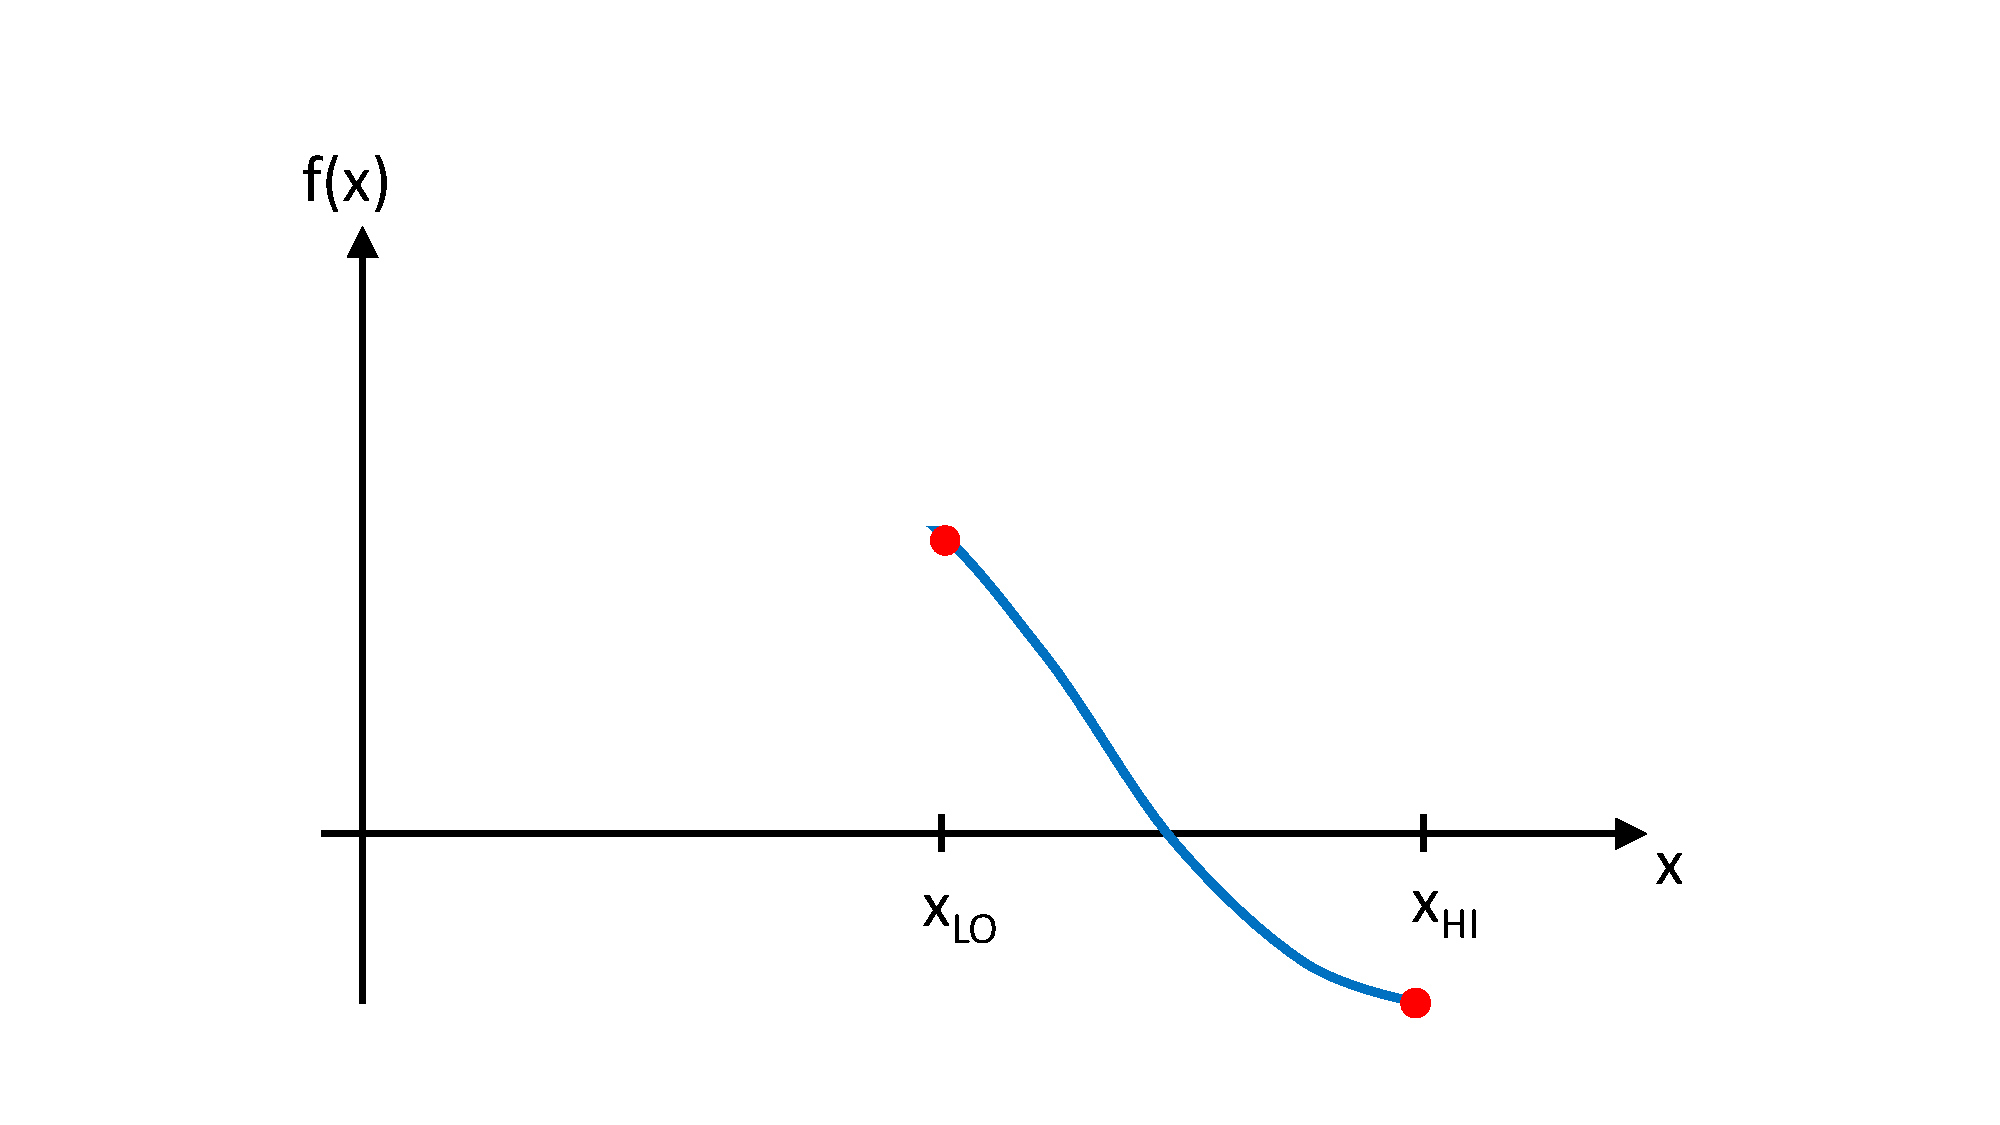
\includegraphics[width=0.8\textwidth]{figures/bisection2}
\end{figure}
\vspace*{-10mm}
\begin{itemize}
\item[] $f(x_\mathrm{MID}) \times f(x_\mathrm{LO}) > 0$
\item[] \ldots select \emph{upper sub-interval} by updating $x_\mathrm{LO} = x_\mathrm{MID}$
\item[] \quad\ldots and repeat
\end{itemize}

\end{frame}

%==============================================================

\begin{frame}[fragile]

\frametitle{Bisection method}

\vspace*{-15mm}
\begin{figure}[ht]
	\centering
	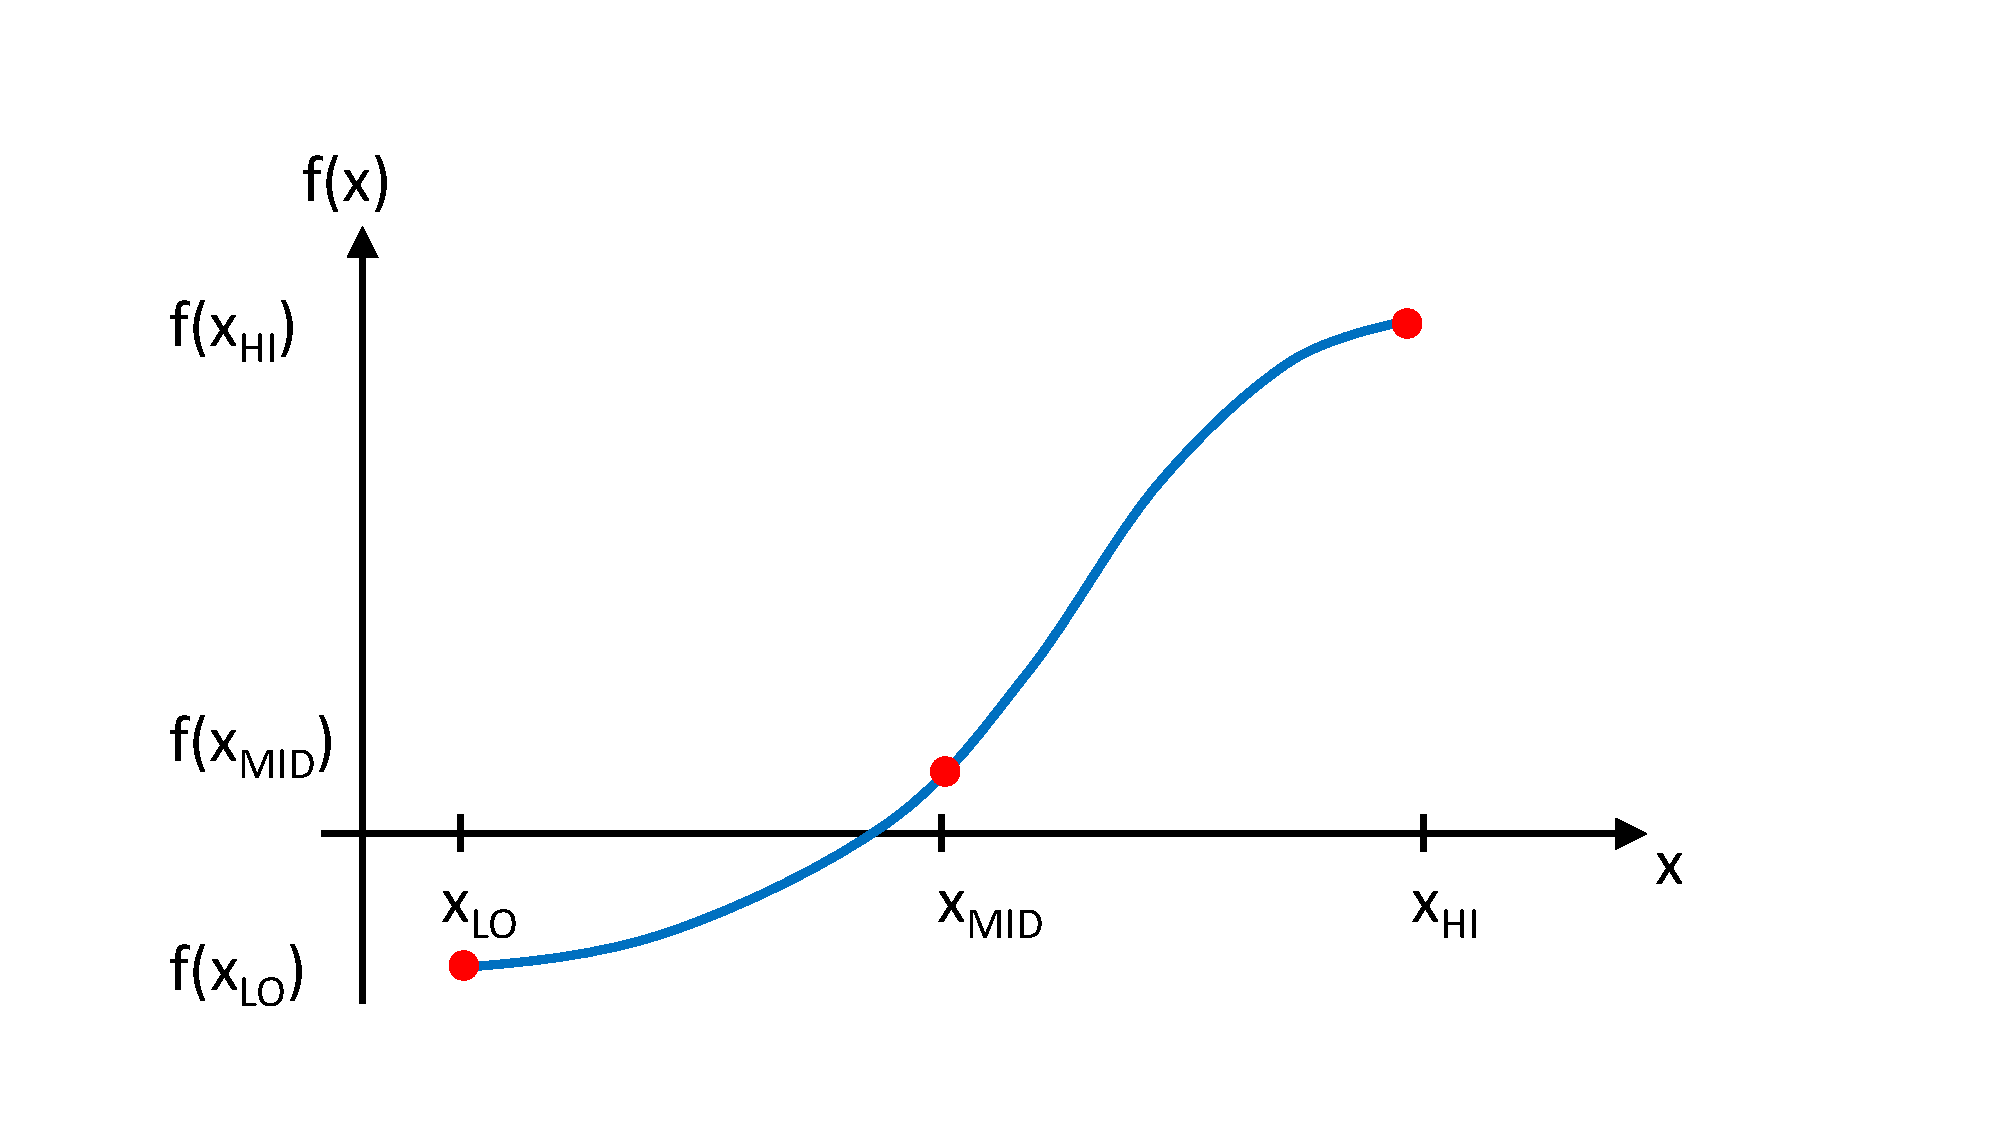
\includegraphics[width=0.8\textwidth]{figures/bisection3}
\end{figure}
\vspace*{-10mm}
\begin{itemize}
\item[] $f(x_\mathrm{MID}) \times f(x_\mathrm{LO}) < 0$
\item[] \ldots select \emph{lower sub-interval} by updating $x_\mathrm{HI} = x_\mathrm{MID}$
\end{itemize}

\end{frame}

%==============================================================

\begin{frame}[fragile]

\frametitle{Bisection method}

\vspace*{-10mm}
\begin{figure}[ht]
	\centering
	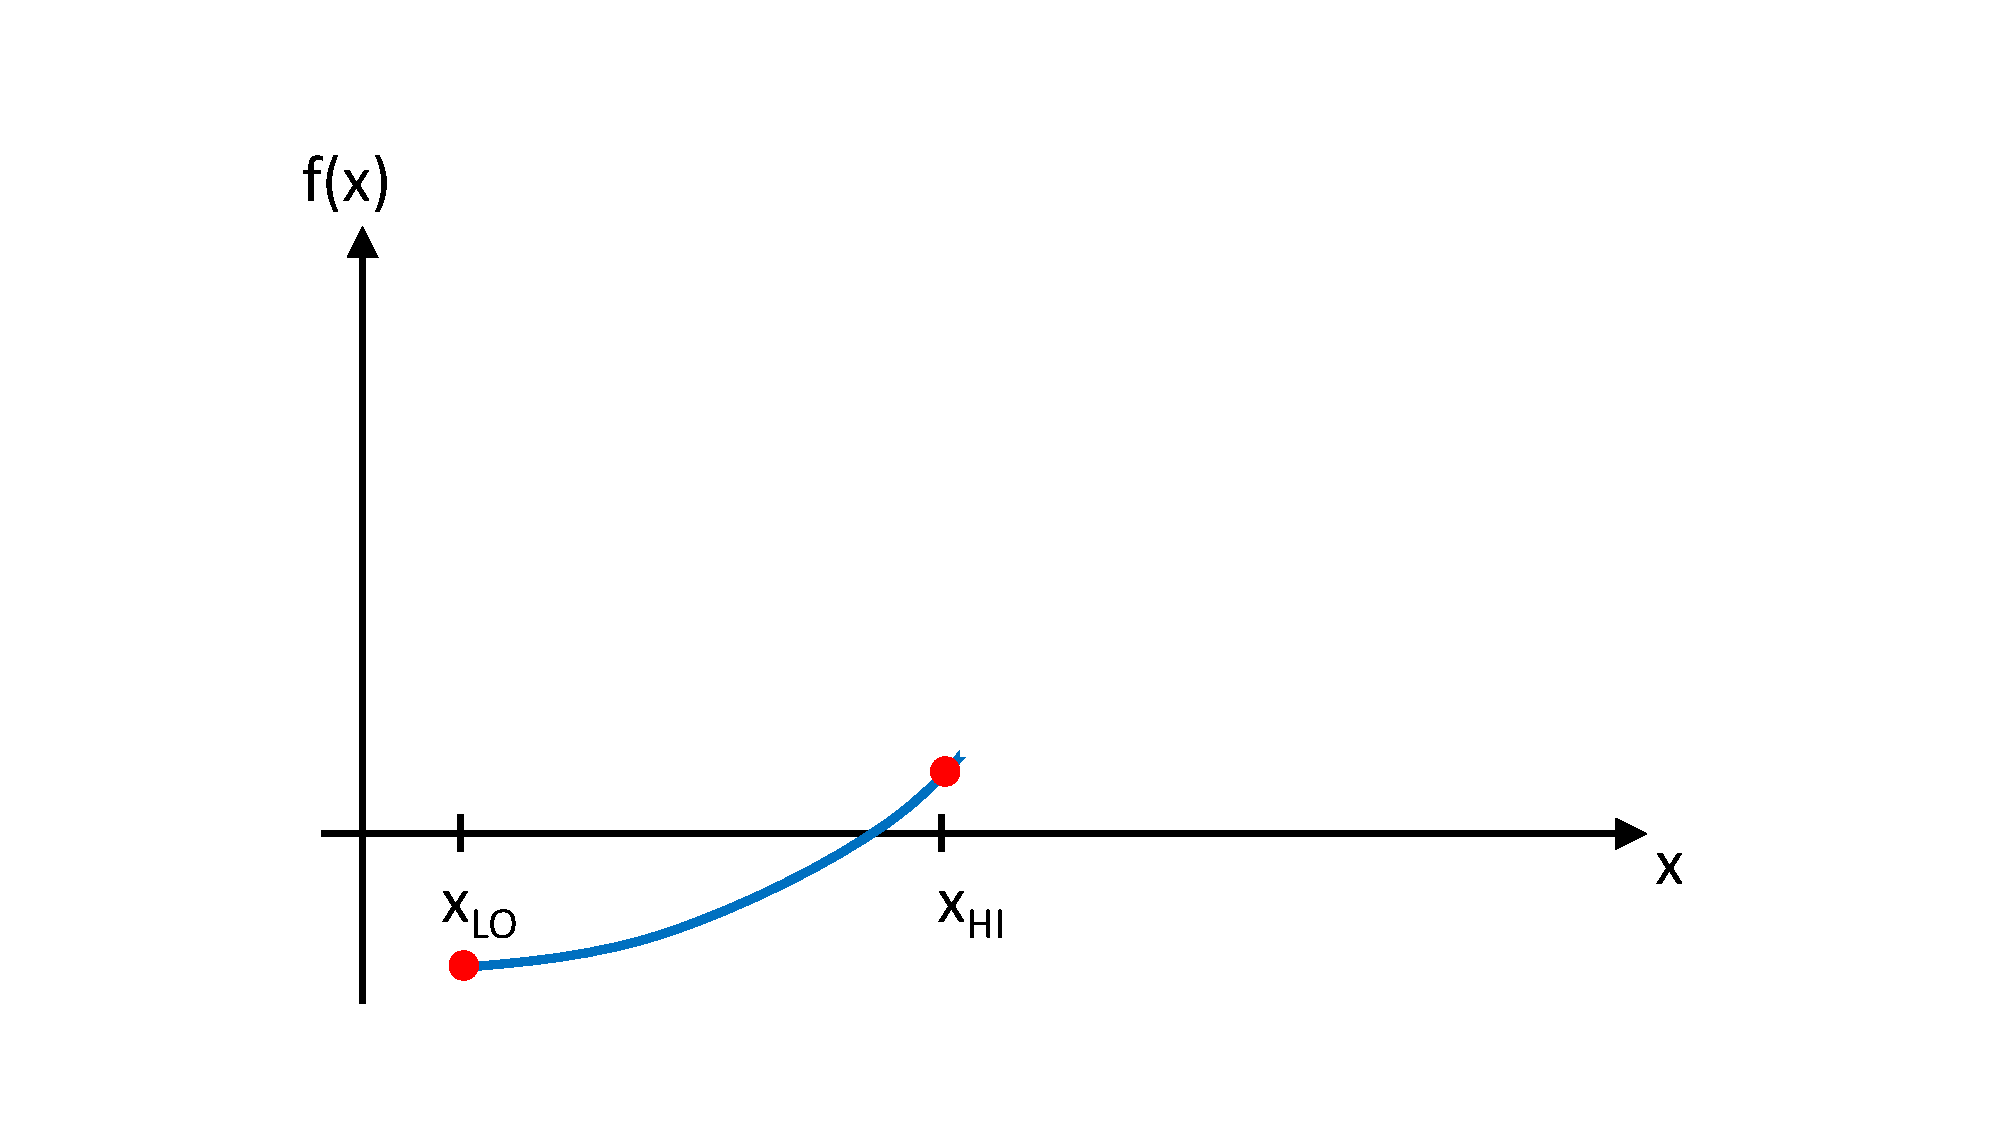
\includegraphics[width=0.8\textwidth]{figures/bisection4}
\end{figure}
\vspace*{-10mm}
\begin{itemize}
\item[] \quad\ldots and repeat, with new midpoint
\[
	x_\mathrm{MID} = (x_\mathrm{LO}+x_\mathrm{HI})/2
\]
\item each iteration halves the width of interval $[x_\mathrm{LO},x_\mathrm{HI}]$
\item continue until $|f(x_\mathrm{MID})| < \mathrm{tolerance}$, eg: $10^{-6}$
\end{itemize}

\end{frame}

%==============================================================

\begin{frame}[fragile]

\frametitle{Bisection method: Python code}
\vspace*{-4mm}
{\small \texttt{bisection.py}}
\vspace*{-2mm}
\begin{lstlisting}[style=CStyle,basicstyle=\scriptsize]
def f(L):
    return  0.0268*L**3 + 1.884*L**2 + 44.15*L - 500

eps = 1e-6
x_LO = 6
x_HI = 10

x_MID = (x_LO + x_HI)/2
itCnt = 0
while abs(f(x_MID)) > eps:
    if f(x_MID)*f(x_LO) > 0:
        x_LO = x_MID
    else:
        x_HI = x_MID
    x_MID = (x_LO + x_HI)/2
    itCnt += 1

print('Solution: {}'.format(x_MID))
print('Number of iterations: {}'.format(itCnt))
print('Check: f({:.8f}) = {:.8f}'.format(x_MID,f(x_MID)))
\end{lstlisting}

\end{frame}

%==============================================================

\begin{frame}[fragile]

\frametitle{Bisection method: simulation results}

\begin{itemize}
	\item lines 1--2: function $f$, want $L$ such that $f(L)=0$
	\item line 4: tolerance $10^{-6}$
	\item lines 9 \& 16: count loop iterations
	\item live demo
\end{itemize}

\begin{figure}[ht]
	\centering
	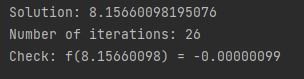
\includegraphics[width=0.8\textwidth]{figures/bisectionOutput}
\end{figure}

\end{frame}

%==============================================================

\begin{frame}[fragile]

\frametitle{$3)$ Secant method}

\vspace*{-15mm}
\begin{figure}[ht]
	\centering
	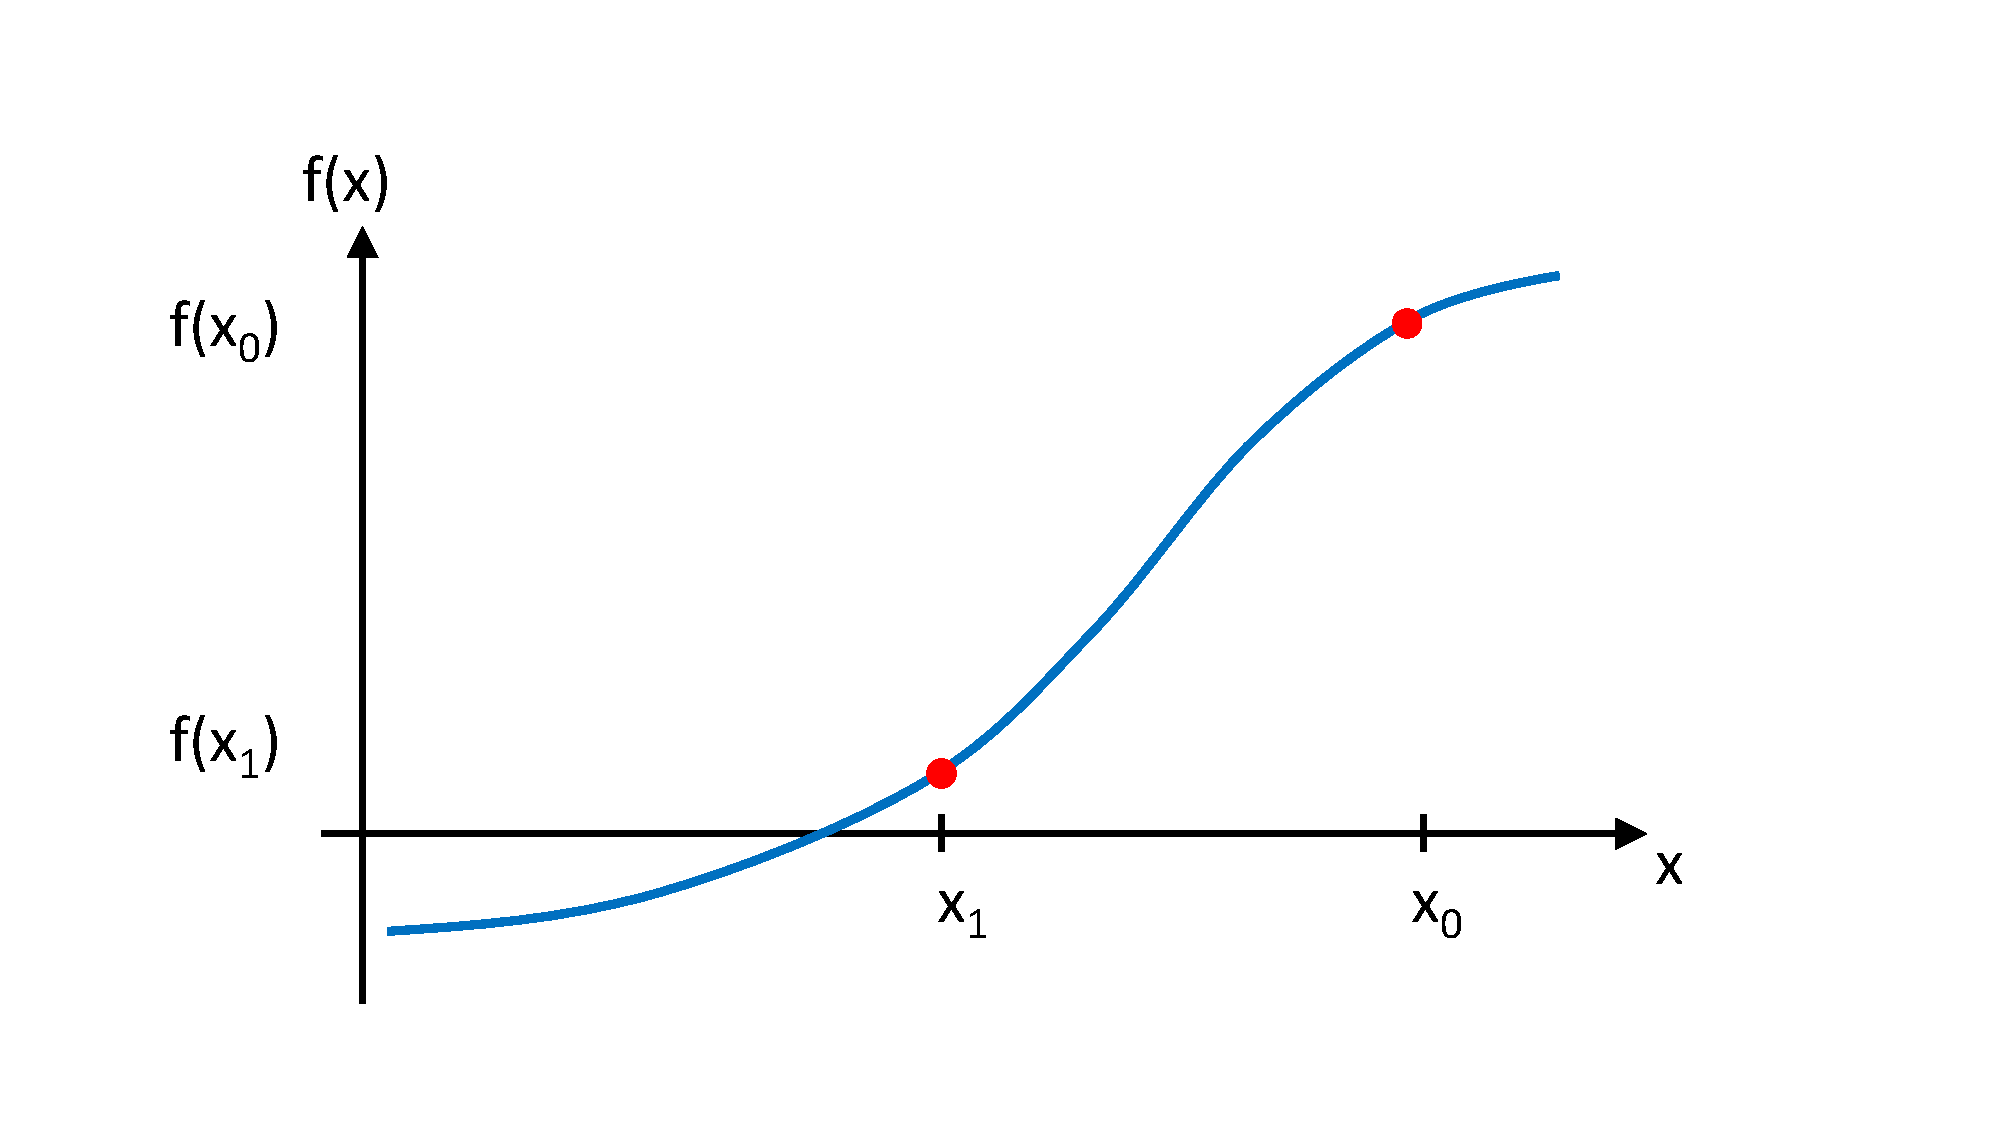
\includegraphics[width=0.8\textwidth]{figures/secant1}
\end{figure}
\vspace*{-10mm}
\begin{itemize}
	\item start with two points $(x_0,f(x_0))$ and $(x_1,f(x_1))$
	\begin{itemize}
		\item \red{red dots}
		\item $f(x_0)$ and $f(x_1)$ do \emph{not} necessarily have opposite signs
	\end{itemize}
\end{itemize}

\end{frame}

%==============================================================

\begin{frame}[fragile]

\frametitle{Secant method}

\vspace*{-15mm}
\begin{figure}[ht]
	\centering
	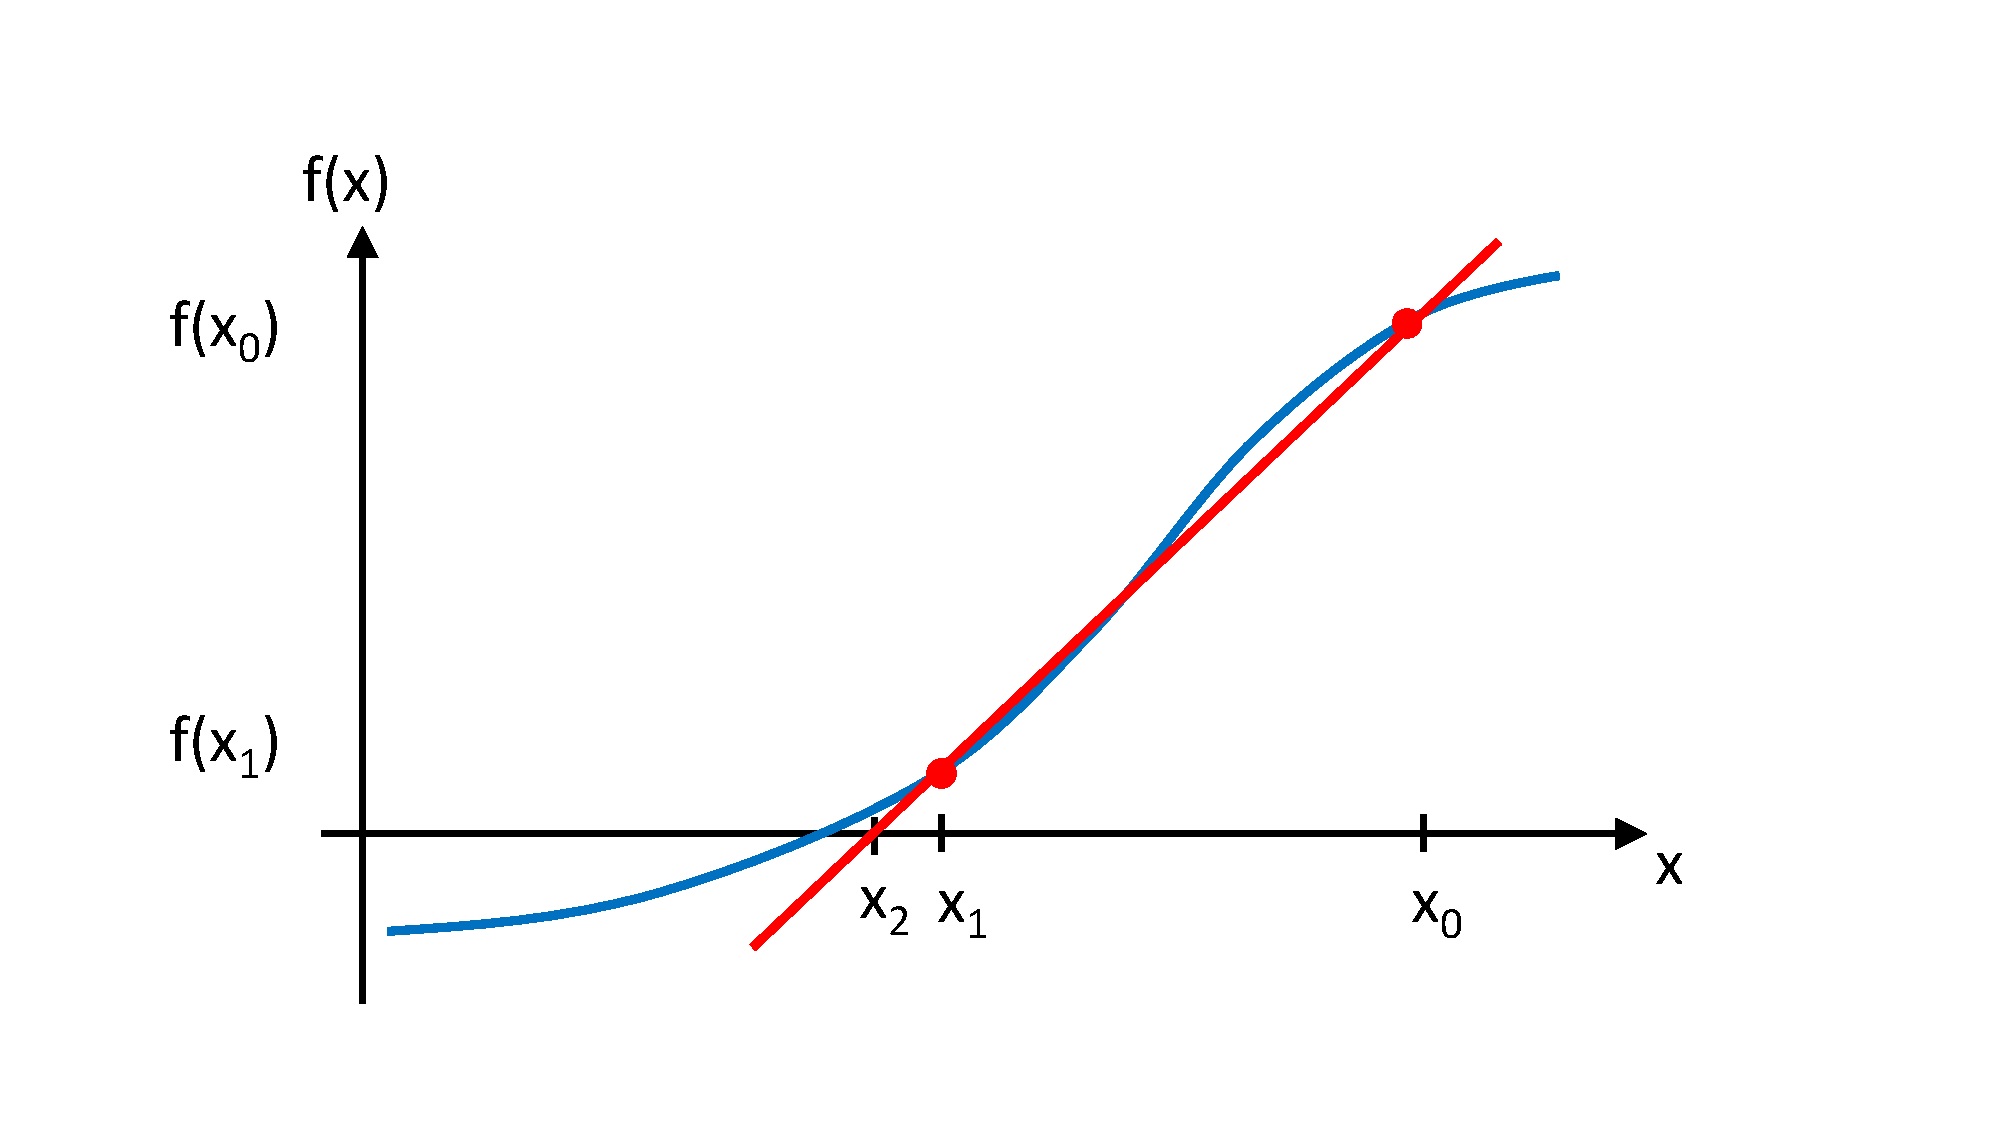
\includegraphics[width=0.8\textwidth]{figures/secant2}
\end{figure}
\vspace*{-10mm}
\begin{itemize}
	\item \emph{\red{secant}} is line through $(x_0,f(x_0))$ and $(x_1,f(x_1))$
	\item define $x_2$ as point where secant intersects $x$-axis
\end{itemize}

\end{frame}

%==============================================================

\begin{frame}[fragile]

\frametitle{Secant method}

\vspace*{-15mm}
\begin{figure}[ht]
	\centering
	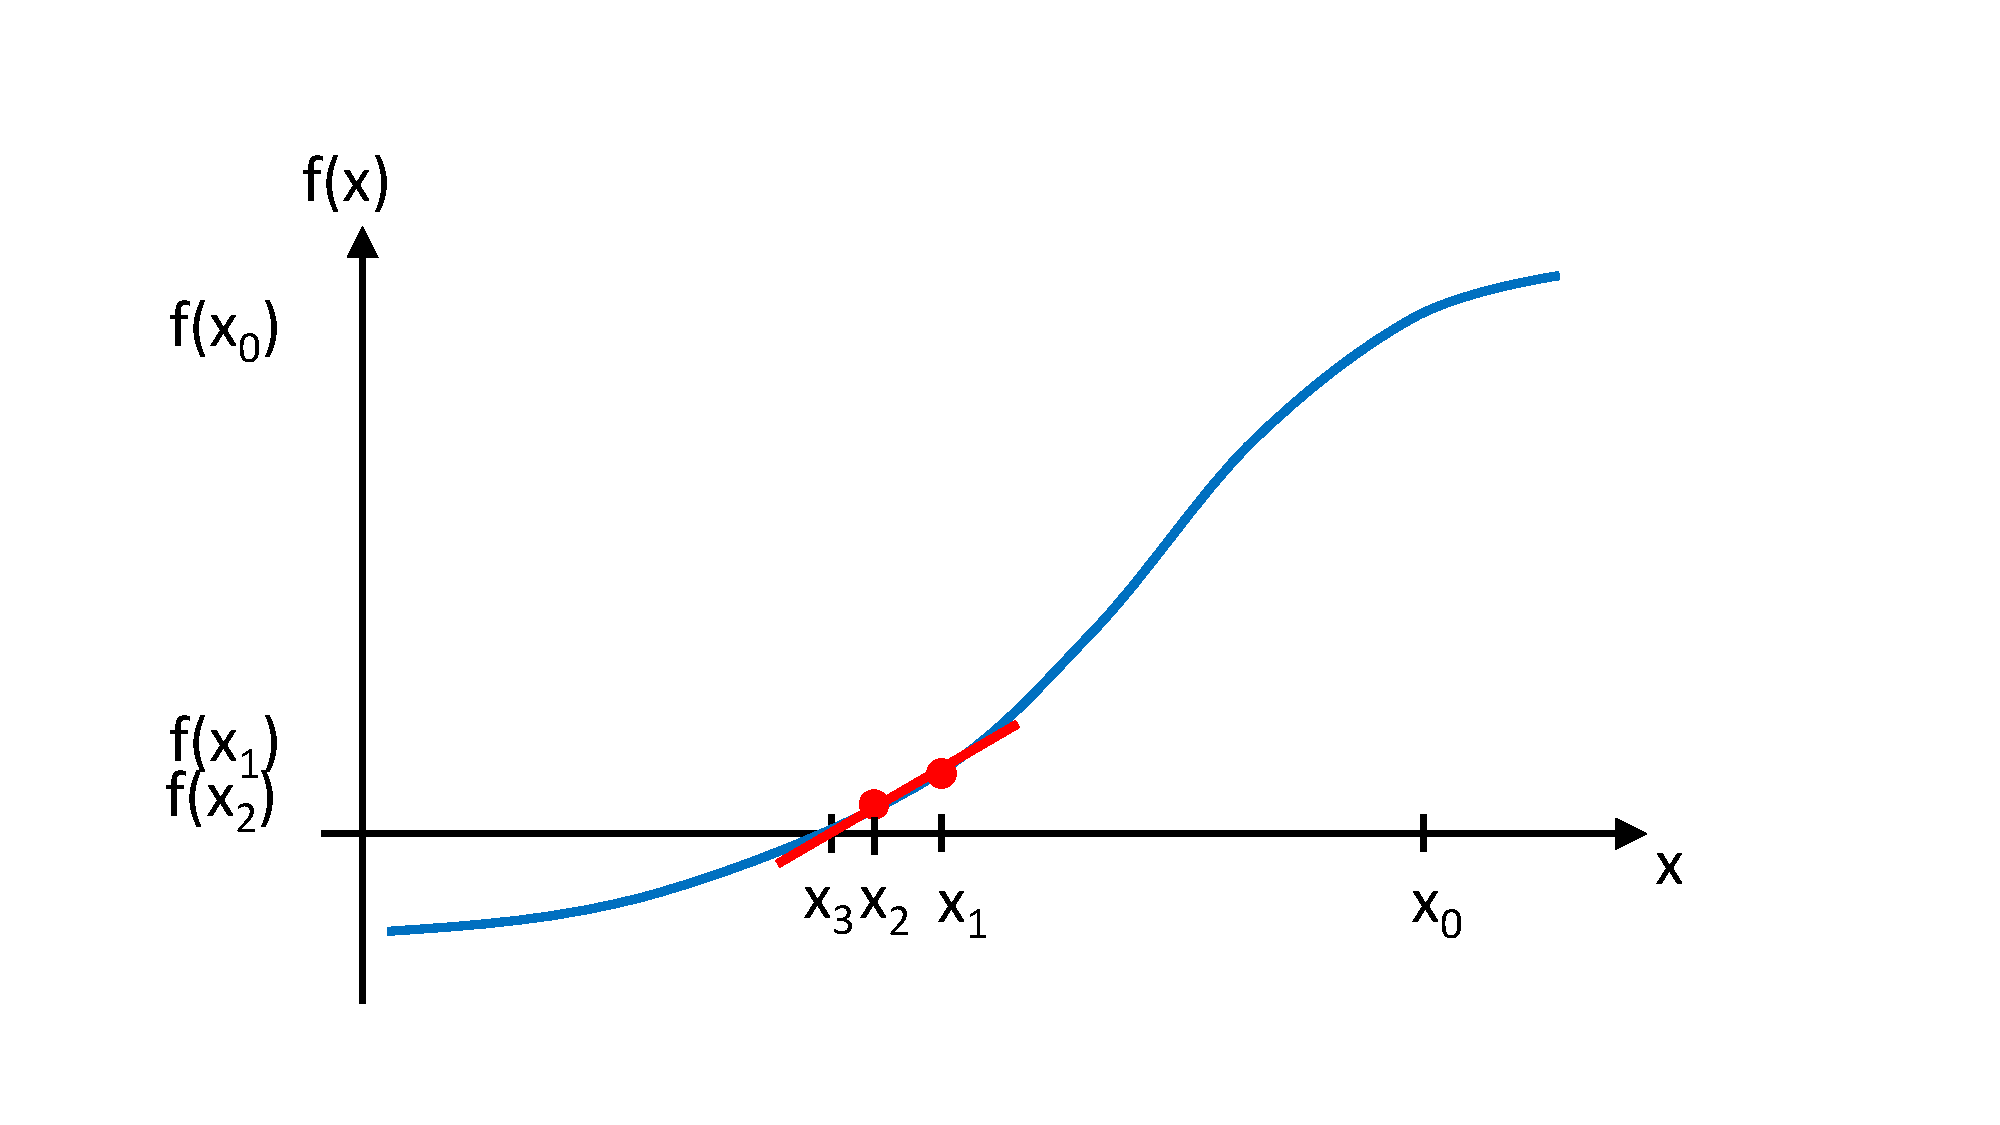
\includegraphics[width=0.8\textwidth]{figures/secant3}
\end{figure}
\vspace*{-10mm}
\begin{itemize}
	\item[] \ldots and repeat, with $x_3$ defined as point where secant through $(x_1,f(x_1))$ and $(x_2,f(x_2))$ intersects $x$-axis
\end{itemize}

\end{frame}

%==============================================================

\begin{frame}[fragile]

\frametitle{Secant method equations}
\vspace*{-2mm}
Equation of secant connecting $(x_0,f(x_0))$ \& $(x_1,f(x_1))$:
\[
	y = \frac{f(x_1)-f(x_0)}{x_1 - x_0}\cdot\left( x - x_1 \right) + f(x_1)
\]
Solving for intersection of secant with $x$-axis:
\[
	x_2 = x_1 - f(x_1)\cdot\frac{x_1 - x_0}{f(x_1) - f(x_0)}
\]
\pause
\[
	x_3 = x_2 - f(x_2)\cdot\frac{x_2 - x_1}{f(x_2) - f(x_1)}
\]
\[
	x_4 = x_3 - f(x_3)\cdot\frac{x_3 - x_2}{f(x_3) - f(x_2)}
\]
\[
	\vdots
\]

\end{frame}

%==============================================================

\begin{frame}[fragile]

\frametitle{Secant method: Python code}

\texttt{secant.py}
\begin{lstlisting}[style=CStyle,basicstyle=\scriptsize]
def f(L):
    return  0.0268*L**3 + 1.884*L**2 + 44.15*L - 500

eps = 1e-6
x0 = 6
x1 = 10
itCnt = 0       # iteration counter
while abs(f(x1)) > eps:
    # line (=secant) through (x0,f(x)) and (x1,f(x1)) intersects
    # horizontal axis at (x,0)
    x = x1 - f(x1)*((x1 - x0)/(f(x1) - f(x0)))
    x0 = x1
    x1 = x
    itCnt += 1

print('Solution: {}'.format(x))
print('Number of iterations: {}'.format(itCnt))
print('Check: f({:.8f}) = {:.8f}'.format(x,f(x)))
\end{lstlisting}

\end{frame}

%==============================================================

\begin{frame}[fragile]

\frametitle{Secant method: simulation results}

\begin{itemize}
	\item lines 12--13: this update simpler to code than $\{x_0, x_1\} \rightarrow x_2$, $\{x_1, x_2\} \rightarrow x_3$, $\{x_2, x_3\} \rightarrow x_4$, \ldots
	\item live demo
\end{itemize}

\begin{figure}[ht]
	\centering
	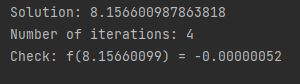
\includegraphics[width=0.8\textwidth]{figures/secantOutput}
\end{figure}

\end{frame}

%==============================================================

\begin{frame}[fragile]

\frametitle{Newton's method}

\vspace*{-6mm}
\begin{figure}[ht]
	\centering
	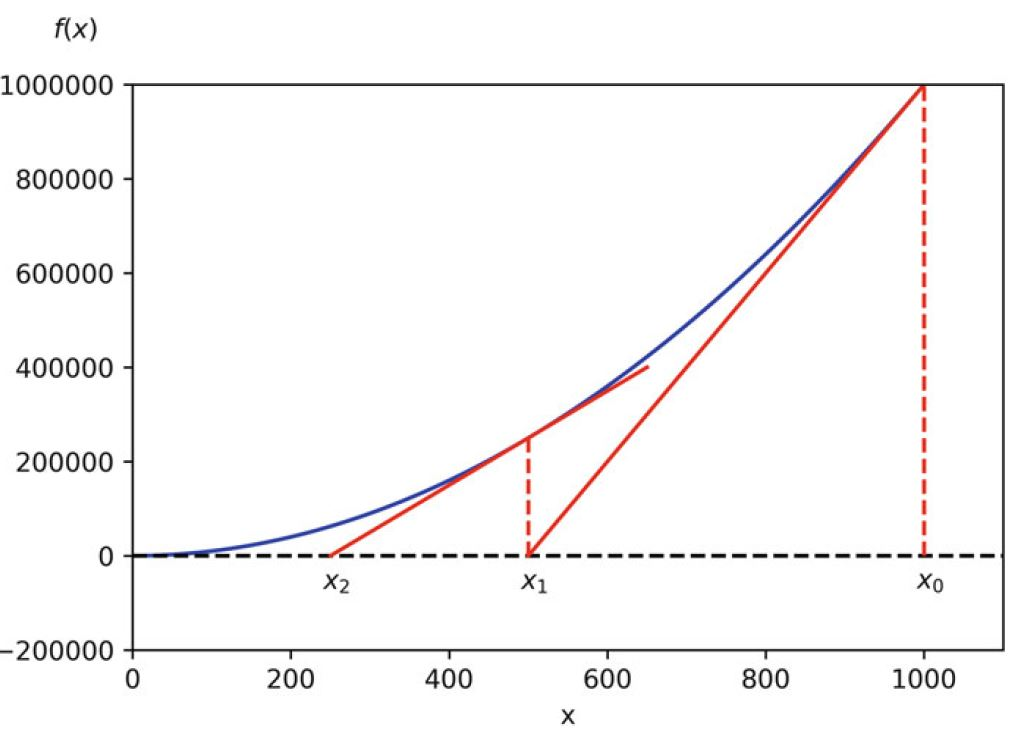
\includegraphics[width=0.55\textwidth]{figures/NewtonsMethod}
\end{figure}
\vspace*{-7mm}
\begin{itemize}
	\item choose initial estimate $x_0$
	\item $x_1$ is intersection of \emph{\red{tangent line}} through $(x_0,f(x_0))$
	\item $x_2$ is intersection of tangent line through $(x_1,f(x_1))$
	\item[] \ldots
\end{itemize}

\end{frame}

%==============================================================

\begin{frame}[fragile]

\frametitle{Newton's method}

\begin{itemize}
	\item also known as \emph{Newton--Raphson method}
	\item Newton's method much more popular than bisection or secant methods
	\item calculation of ``tangent lines'' requires \emph{\red{derivative}} of function $f(x)$
	\begin{itemize}
		\item therefore needs \emph{calculus} (eg: MATH1110)
		\item beyond assumed knowledge for ENGG1003, won't consider Newton's method in this course
	\end{itemize}
	\item secant method can be considered as an approximation to Newton's method
\end{itemize}

\end{frame}

%==============================================================

\begin{frame}[fragile]

\frametitle{$4)$ Extensions}

\texttt{bisection\_fn.py}
\begin{lstlisting}[style=CStyle,basicstyle=\scriptsize]
def f(L):
    return 0.0268*L**3 + 1.884*L**2 + 44.15*L - 500

def my_bisection(f, x_LO, x_HI, tol):
    x_MID = (x_LO + x_HI) / 2
    itCnt = 0
    while abs(f(x_MID)) > tol:
        if f(x_MID) * f(x_LO) > 0:
            x_LO = x_MID
        else:
            x_HI = x_MID
        x_MID = (x_LO + x_HI) / 2
        itCnt += 1
    return x_MID, itCnt

x, numIt = my_bisection(f, 4, 12, 1e-6)

print('Solution: {}'.format(x))
print('Number of iterations: {}'.format(numIt))
print('Check: f({:.8f}) = {:.8f}'.format(x,f(x)))
\end{lstlisting}

\end{frame}

%==============================================================

\begin{frame}[fragile]

\frametitle{Bisection method as a function}

\begin{itemize}
	\item line 4: \texttt{my\_bisection} function takes function \texttt{f} as first argument
	\item[] \ldots also pass in $x_\mathrm{LO}$, $x_\mathrm{HI}$ and convergence tolerance
	\item[]
	\item line 14: function returns approximate solution \& iteration count
	\item[]
	\item line 16: call \texttt{my\_bisection} function with four arguments
	\item[]
	\item live demo
\end{itemize}

\end{frame}

%==============================================================

\begin{frame}[fragile]

\frametitle{Secant method as a function}

\texttt{secant\_fn.py}
\begin{lstlisting}[style=CStyle,basicstyle=\scriptsize]
def f(L):
    return 0.0268*L**3 + 1.884*L**2 + 44.15*L - 500

def my_secant(f, x0, x1, tol):
    itCnt = 0
    while abs(f(x1)) > tol:
        x = x1 - f(x1) * ((x1 - x0) / (f(x1) - f(x0)))
        x0 = x1
        x1 = x
        itCnt += 1
    return x1, itCnt

x, numIt = my_secant(f, 4, 12, 1e-8)

print('Solution: {}'.format(x))
print('Number of iterations: {}'.format(numIt))
print('Check: f({:.8f}) = {:.8f}'.format(x,f(x)))
\end{lstlisting}

\begin{itemize}
	\item live demo
\end{itemize}

\end{frame}

%==============================================================

\begin{frame}[fragile]

\begin{itemize}
	\item often useful to measure time taken to perform calculations; easy in Python!
	\item start by importing \texttt{time} module:
\end{itemize}

\frametitle{Timing code in Python}
\begin{lstlisting}[style=CStyle,basicstyle=\scriptsize]
import time
\end{lstlisting}

\begin{itemize}
	\item function \texttt{time.perf\_counter()} returns value of a clock
	\begin{itemize}
		\item \texttt{float} value (in seconds) 
	\end{itemize}
	\item elapsed time is \emph{difference} between two successive calls
\end{itemize}

\begin{lstlisting}[style=CStyle,basicstyle=\scriptsize]
tStart = time.perf_counter()
xB, numItB = my_bisection(f, 6, 10, 1e-6)
tStop = time.perf_counter()
tBisect = tStop - tStart
\end{lstlisting}

\end{frame}

%==============================================================

\begin{frame}[fragile]

\frametitle{Speed comparison: bisection vs.~secant}

\begin{itemize}
	\item live demo \texttt{bisectionvssecant.py}
	\item code in \#lecturecode
\end{itemize}

\begin{figure}[ht]
	\centering
	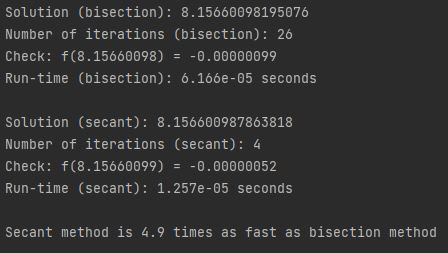
\includegraphics[width=0.8\textwidth]{figures/BisectionSecantSpeed}
\end{figure}

\end{frame}

%==============================================================

\begin{frame}[fragile]

\frametitle{Lecture summary}
\begin{itemize}
	\item Solving nonlinear algebraic equations

	\item[]
	
	\item Bisection method

	\item[]
	
	\item Secant method
	\begin{itemize}
		\item Newton's method
	\end{itemize}

	\item[]
	
	\item Extensions
	
\end{itemize}

\end{frame}

%==============================================================

\begin{frame}[fragile]

\frametitle{More information}
\begin{itemize}
	\item Newton's method in textbook \red{\S7.2}
	\begin{itemize}
		\item needs \emph{differentiation} from calculus (MATH1110)
		\item in particular: need expression for \emph{tangent lines} to function $f(x)$, written as $f'(x)$
	\end{itemize}

	\item[]
	
	\item ``optimised'' versions of bisection and secant methods in textbook \red{\S7.3} and \red{\S7.4}
	\begin{itemize}
		\item maximise speed of computation by minimising number of function evaluations $f(x)$
	\end{itemize}
	
	\item[]
	
	\item volume of truncated cone based on volumes of solids of revolution (needs calculus, MATH1110) \href{https://bit.ly/3sOsaj4}{https://bit.ly/3sOsaj4}
\end{itemize}

\end{frame}

\end{document}